\documentclass[10pt,twocolumn]{article}
\usepackage[utf8]{inputenc}
\usepackage[T1]{fontenc}
\usepackage[margin=0.68in]{geometry}
\usepackage{amsmath,amssymb}
\usepackage{booktabs}
\usepackage{graphicx}
\usepackage{hyperref}
\usepackage{array}
\usepackage{caption}

\hypersetup{
    colorlinks=true,
    linkcolor=blue,
    citecolor=blue,
    urlcolor=blue
}

\setlength{\columnsep}{0.24in}
\captionsetup{font=footnotesize,labelfont=bf}

\title{\textbf{MedTRT: Eliminating End-to-End I/O, Resampling, and FP16 Quantization Bottlenecks in 3D CT Organ Segmentation}}
\author{\textbf{Diego D\'iaz Rivera}\\
Biomedical AI Systems \& GPU Performance Engineering\\
\texttt{MedTRT Research Study (NVIDIA GeForce RTX 5080 Blackwell sm\_120)}}
\date{November 6, 2026}

\begin{document}
\maketitle

\begin{abstract}
\noindent\textbf{Problem:} Deploying 3D convolutional neural networks for volumetric computed tomography (CT) segmentation is widely assumed to be compute-bound by the neural network forward pass. Profiling a pretrained MONAI 3D Residual U-Net (\texttt{spleen\_ct\_segmentation} v0.6.1) across $53$ abdominal CT volumes ($41$ Medical Segmentation Decathlon \texttt{Task09\_Spleen} scans plus $12$ external multi-center MICCAI \texttt{FLARE22} scans archived on Google Drive) reveals two critical bottlenecks. First, by Amdahl's Law, the 3D U-Net forward pass ($254.6\text{ ms}$) accounts for only $8.6\%$ of the $2,952.0\text{ ms}$ host-path end-to-end latency; $91.4\%$ is consumed by CPU trilinear inverse resampling ($1,990.4\text{ ms}$), \texttt{.nii.gz} decompression ($424.7\text{ ms}$), and CPU spatial resampling ($286.4\text{ ms}$). Moving spatial transforms to MONAI's GPU \texttt{grid\_sample} backend ($215.5\text{ ms}$) allocates dense \texttt{float64} 3D coordinate meshgrids requiring $2,301\text{ MB}$ of VRAM ($5.1\times$ larger than the network). Second, compiling the exported ONNX graph directly into TensorRT FP16 introduces a systematic volumetric over-segmentation bias of $+1.675 \pm 0.553\text{ cm}^3$ ($9/9$ internal scans, $p < 0.0001$) and $+1.537 \pm 0.768\text{ cm}^3$ ($12/12$ external scans) caused by an unfused decoder \texttt{ConvTranspose3d+BatchNorm3d} pair (\texttt{model.2.0.adn.N}) where an affine shift of $-81.79$ at $\text{ULP}_{\text{FP16}} = 0.0625$ induces catastrophic floating-point cancellation.

\smallskip
\noindent\textbf{Approach:} Around the frozen public weights, we engineered: (1) an analytical \texttt{float64} pre-export weight transformation that algebraically folds \texttt{BatchNorm3d} into \texttt{ConvTranspose3d} prior to ONNX export and TensorRT 10.16 FP16 compilation; (2) nine custom CUDA C++17 3D kernels (\texttt{sm\_120}) that compute $3 \times 4$ voxel-to-voxel affine coordinates directly in registers via fused multiply-add (\texttt{\_\_fmaf\_rn}), eliminating 3D coordinate meshgrids and fusing Hounsfield Unit windowing ($1.27\text{ ms}$) and trilinear postprocessing ($2.62\text{ ms}$); and (3) a zero-copy TensorRT execution engine paired with OS page-cache memory-mapped (\texttt{mmap}) \texttt{.nii} ingestion.

\smallskip
\noindent\textbf{Results:} Under identical sliding-window settings ($\text{overlap}=0.5, B=4$), our like-for-like custom CUDA + TensorRT FP16 pipeline (\texttt{trt\_fp16\_cuda}) reduces median end-to-end latency from $2,952.0\text{ ms}$ to $\mathbf{96.3\textbf{ ms}}$ ($\mathbf{30.7\times}$ cohort median speedup; paired patient-level mean speedup $\mathbf{33.1\times}$, $95\%$ CI $[27.6\times, 38.7\times]$) and cuts peak VRAM from $2,301\text{ MB}$ to $\mathbf{455\textbf{ MB}}$ ($\mathbf{5.1\times}$ reduction). A fast sliding-window profile (\texttt{trt\_fp16\_optimized}, $\text{overlap}=0.25, B=8$) reaches $\mathbf{68.9\textbf{ ms}}$ median latency ($\mathbf{42.9\times}$ cohort speedup; paired patient-level median $\mathbf{46.6\times}$). Analytical \texttt{ConvTranspose3d+BatchNorm3d} folding reduces mean absolute logit error by $\mathbf{35.6\times}$ and achieves near-FP32 segmentation agreement under the evaluated conditions: across the pooled $N = 21$ internal and external validation patients, paired Two One-Sided Tests (TOST) establish statistical equivalence within $\Delta_V = \pm 0.10\text{ cm}^3$ (mean bias $-0.0059 \pm 0.0271\text{ cm}^3$, $90\%$ CI $[-0.0161, +0.0043]\text{ cm}^3$, $p_{\text{TOST}} < 10^{-6}$) and $\Delta_{\text{Dice}} = \pm 0.001$ ($p_{\text{TOST}} < 10^{-6}$), with only $0.009\%$ ($8.8/95,529$) of organ voxels flipping label on internal scans and $0.019\%$ ($23.2/167,879$) on unseen external \texttt{FLARE22} scans.
\end{abstract}

\section{Introduction \& Problem Identification}
Three-dimensional convolutional architectures such as the 3D Residual U-Net \cite{kerfoot2019,cicek2016} are standard backbones for volumetric CT organ segmentation. Because an abdominal CT volume ($512 \times 512 \times 31\text{--}135$ voxels) exceeds typical GPU memory if processed monolithically, clinical research pipelines in MONAI \cite{cardoso2022} reorient the volume to RAS coordinates, resample to canonical spacing ($1.5 \times 1.5 \times 2.0\text{ mm}$), execute sliding-window inference over overlapping $96 \times 96 \times 96$ patches, and invert the resampled probability volume back to native scanner coordinates.

Profiling the public MONAI \texttt{spleen\_ct\_segmentation} v0.6.1 bundle \cite{monaibundle2024,xia2018} on the Medical Segmentation Decathlon (MSD) \texttt{Task09\_Spleen} dataset \cite{antonelli2022,simpson2019} and the external multi-center MICCAI \texttt{FLARE22} dataset \cite{ma2023flare} on an NVIDIA GeForce RTX 5080 Laptop GPU (Blackwell \texttt{sm\_120}) exposed three systems and numerical obstacles:
\begin{enumerate}
    \item \textbf{Amdahl's Law Non-Network Bottleneck ($91.4\%$ of Runtime):} In the baseline host pipeline (\texttt{pytorch\_fp32}), end-to-end median latency is $2,952.0\text{ ms}$, whereas the 3D U-Net forward pass (\texttt{sw\_network}) takes only $254.6\text{ ms}$ ($8.6\%$). By Amdahl's Law \cite{amdahl1967}, $S_{\max} = (1 - 0.0862)^{-1} = 1.094\times$. Replacing PyTorch with TensorRT FP16 on the host path (\texttt{trt\_fp16}) lowers network time to $167.1\text{ ms}$ but yields only a $1.02\times$ end-to-end speedup ($2,880.3\text{ ms}$) because CPU trilinear \texttt{Invertd} ($1,993.9\text{ ms}$), \texttt{.nii.gz} decompression ($385.1\text{ ms}$), and CPU \texttt{Spacingd} ($266.8\text{ ms}$) dominate execution and allow the laptop GPU to downclock to $180\text{ MHz}$ (\texttt{P4}) between scans ($2.34\times$ idle clock penalty).
    \item \textbf{MONAI GPU Meshgrid VRAM Overhead ($2,301\text{ MB}$):} Moving transforms onto the GPU via MONAI's \texttt{grid\_sample} backend (\texttt{trt\_fp16\_gpu}) reduces median latency to $215.5\text{ ms}$ but allocates dense \texttt{float64} 3D coordinate meshgrids $(1, D, H, W, 3)$, inflating peak VRAM to $2,301.3\text{ MB}$. Inverting discretized labels via nearest-neighbor interpolation (\texttt{trt\_fp16\_nn}) degrades mean Dice by $-0.0050$ ($0.960230$ vs.\ $0.965233$).
    \item \textbf{Systematic FP16 Volumetric Drift ($+1.68\text{ cm}^3$):} Compiling the exported ONNX graph directly into TensorRT FP16 (\texttt{trt\_fp16\_unfolded}) inflates segmented spleen volume by $+1.6754 \pm 0.5531\text{ cm}^3$ ($p < 0.0001$) on $9/9$ internal MSD scans and $+1.5366 \pm 0.7680\text{ cm}^3$ ($p < 0.0001$) on $12/12$ external \texttt{FLARE22} scans. Layer-by-layer inspection revealed that PyTorch's ONNX exporter folds \texttt{BatchNorm3d} into \texttt{Conv3d} in the encoder, but leaves \texttt{BatchNorm3d} unfused after \texttt{ConvTranspose3d} in the decoder. In layer \texttt{model.2.0.adn.N}, \texttt{ConvTranspose3d} activations average $\mu = 57.62$ before \texttt{BatchNorm3d} applies an affine shift of $-81.79$. In IEEE-754 FP16 (10-bit significand), values in $[64, 128)$ have $\text{ULP} = 2^{-4} = 0.0625$, causing catastrophic cancellation that shifts background logits by $-0.159$ and foreground logits by $+0.116$.
\end{enumerate}

\section{Experimental Setup \& Methodology}

\subsection{Hardware, Power Limits, \& Timing Protocol}
All experiments executed on a single workstation equipped with an \textbf{NVIDIA GeForce RTX 5080 Laptop GPU} (Blackwell architecture, compute capability $12.0$ / \texttt{sm\_120}, $15.92\text{ GB}$ GDDR7 VRAM, $90\text{ W}$ dynamic TGP limit under Windows 11 build \texttt{10.0.26300} in \texttt{WDDM} driver mode, NVIDIA Driver \texttt{591.44}, CUDA \texttt{12.8}, cuDNN \texttt{9.19.0}, TensorRT \texttt{10.16.1.11}, PyTorch \texttt{2.11.0+cu128}, MONAI \texttt{1.6.1}, and Python \texttt{3.11.15}). Active GPU execution runs in performance state \texttt{P0} ($1,500+\text{ MHz}$ graphics clock), whereas host-bound stalls over $2\text{ s}$ allow hardware power management to drop to \texttt{P4} ($180\text{ MHz}$).

Each benchmark profile executes $3$ untimed warm-up volumes (stabilizing \texttt{P0} clocks, cuDNN autotuning, and CUDA allocator pools) followed by $10$ timed passes across each of the $9$ internal validation volumes ($90$ timed passes per profile). Stage boundaries (\texttt{load}, \texttt{h2d}, \texttt{preprocess}, \texttt{sw\_network}, \texttt{sw\_aggregate}, \texttt{postprocess}, and \texttt{e2e\_total}) are bracketed by hardware \texttt{torch.cuda.Event(enable\_timing=True)} pairs synchronized via \texttt{torch.cuda.synchronize()} and cross-checked against host \texttt{time.perf\_counter()} wall-clock timers (worst median discrepancy across all 13 profiles: $0.26\%$). Every timed pass ends with the discretized \texttt{uint8} 3D segmentation mask transferred back to host RAM.

\subsection{Ingestion Modes \& Stage-Sum Accounting}
We distinguish three I/O regimes measured across the 9 MSD volumes ($31\text{--}135\text{ MB}$ uncompressed): (1) \textbf{CPU \texttt{.nii.gz} gzip decompression} ($265.0\text{ ms}$ standalone median; $385.1\text{--}424.7\text{ ms}$ inside the full host pipeline), (2) \textbf{cold unbuffered \texttt{.nii} disk reads} (\texttt{open(..., buffering=0)}, $23.8\text{ ms}$ median on local NVMe), and (3) \textbf{warm OS page-cache memory mapping} (\texttt{nibabel.load(..., mmap=True)}, where \texttt{load} takes $1.5\text{ ms}$ to construct the virtual mapping and the page-cached bytes are faulted directly during the $27.6\text{ ms}$ host-to-device copy, yielding $\text{ingest} = \text{load} + \text{h2d} = 29.2\text{ ms}$ median on local NVMe and $175.4\text{ ms}$ over the virtualized Google Drive mount).

Crucially, in tables reporting medians across heterogeneous CT volumes ($31$ to $135$ slices, $32$ to $125$ sliding windows), the sum of marginal stage medians is mathematically distinct from the median of end-to-end sums ($\sum_k \text{median}(T_k) \neq \text{median}(\sum_k T_k)$), and omitting \texttt{ingest} ($29.2\text{ ms}$) and \texttt{sw\_aggregate} ($6.1\text{ ms}$) creates an apparent gap between compute stages ($1.3 + 49.0 + 2.6 = 52.9\text{ ms}$) and total latency ($96.3\text{ ms}$). Table~\ref{tab:master} therefore reports all six pipeline stages explicitly, where the sum of all six stage medians on \texttt{trt\_fp16\_cuda} is $29.2 + 1.3 + 49.0 + 6.1 + 2.6 = 88.2\text{ ms}$ vs.\ $96.3\text{ ms}$ median E2E (within single-case medians, e.g.\ \texttt{spleen\_59}, the six stages sum to $24.8 + 1.3 + 54.3 + 6.7 + 2.1 = 89.2\text{ ms}$ vs.\ $89.7\text{ ms}$ E2E).

\subsection{Two-Cohort Validation Design \& Statistical Rigor}
To separate repeated-pass timing precision ($90$ passes) from patient-level biological variation ($N$ independent subjects), all accuracy, volumetric bias, and paired speedup confidence intervals are computed at the \textbf{patient level}:
\begin{itemize}
    \item \textbf{Cohort 1 (Internal MSD \texttt{Task09\_Spleen}, $N = 9$ validation / $41$ total CT scans):} Following \texttt{configs/train.json} (\texttt{@images[-9:]}), the final 9 alphanumerically sorted volumes (\texttt{spleen\_56} to \texttt{spleen\_9}) form the held-out split. While disjoint from the 32 gradient-update scans, the bundle's \texttt{CheckpointSaver} selected \texttt{model.pt} using validation Dice on these 9 scans; thus absolute Dice ($0.9652$) is an optimistic internal estimate, whereas cross-backend comparisons against strict IEEE FP32 (\texttt{pytorch\_fp32\_strict}) are exact. All $41$ MSD volumes are also benchmarked on GPU ($68.9\text{ ms}$ median on $N=9$; $90.4\text{ ms}$ across all $N=41$).
    \item \textbf{Cohort 2 (External Unseen MICCAI \texttt{FLARE22}, $N = 12$ multi-center CT scans on Google Drive):} To provide an unbiased external test of both generalization and numerical equivalence, we curated $12$ independent abdominal CT scans (\texttt{FLARE22\_Tr\_0001} to \texttt{0012}, $512 \times 512 \times 84\text{--}110$ voxels, spacing $0.64\text{--}0.86 \times 2.5\text{ mm}$, ground-truth spleen volumes $130.8\text{--}481.7\text{ cm}^3$) from the official MICCAI FLARE22 dataset (Zenodo Record \texttt{7860267} \cite{ma2023flare}), archived persistently on Google Drive (\texttt{MedTRT\_Datasets/FLARE22\_External\_Cohort}).
    \item \textbf{Formal TOST Equivalence Testing:} Because a non-significant two-sided $t$-test ($p = 0.885$) only fails to reject a zero difference and cannot prove equivalence, we perform paired \textbf{Two One-Sided Tests (TOST)} \cite{schuirmann1987} at $\alpha = 0.05$ against predefined equivalence margins of $\Delta_V = \pm 0.10\text{ cm}^3$ ($< 0.05\%$ of mean spleen volume) and $\Delta_V = \pm 0.50\text{ cm}^3$, and $\Delta_{\text{Dice}} = \pm 0.001$ and $\pm 0.005$.
\end{itemize}

\section{Engineering \& Numerical Solutions}

\subsection{Analytical FP64 \texttt{ConvTranspose3d+BN} Folding}
Prior to ONNX (\texttt{opset 17}) export \cite{onnx2019}, we algebraically fold each decoder \texttt{BatchNorm3d} ($\gamma, \beta, \mu, \sigma^2, \epsilon$) into its preceding \texttt{ConvTranspose3d} weight $W$ and bias $b$ in \texttt{float64}:
\begin{equation}
\begin{gathered}
s_c = \frac{\gamma_c}{\sqrt{\sigma_c^2 + \epsilon}}, \quad \widetilde{W}_{:, c, :, :, :} = W_{:, c, :, :, :} \cdot s_c, \\
\widetilde{b}_c = (b_c - \mu_c)s_c + \beta_c
\end{gathered}
\end{equation}
and replace \texttt{BatchNorm3d} with \texttt{Identity()}. In FP32, this alters logits by at most $1.34 \times 10^{-5}$, while eliminating the $-81.79$ intermediate shift prior to FP16 quantization in TensorRT 10.16 \cite{tensorrt2025}.

\begin{figure}[t]
    \centering
    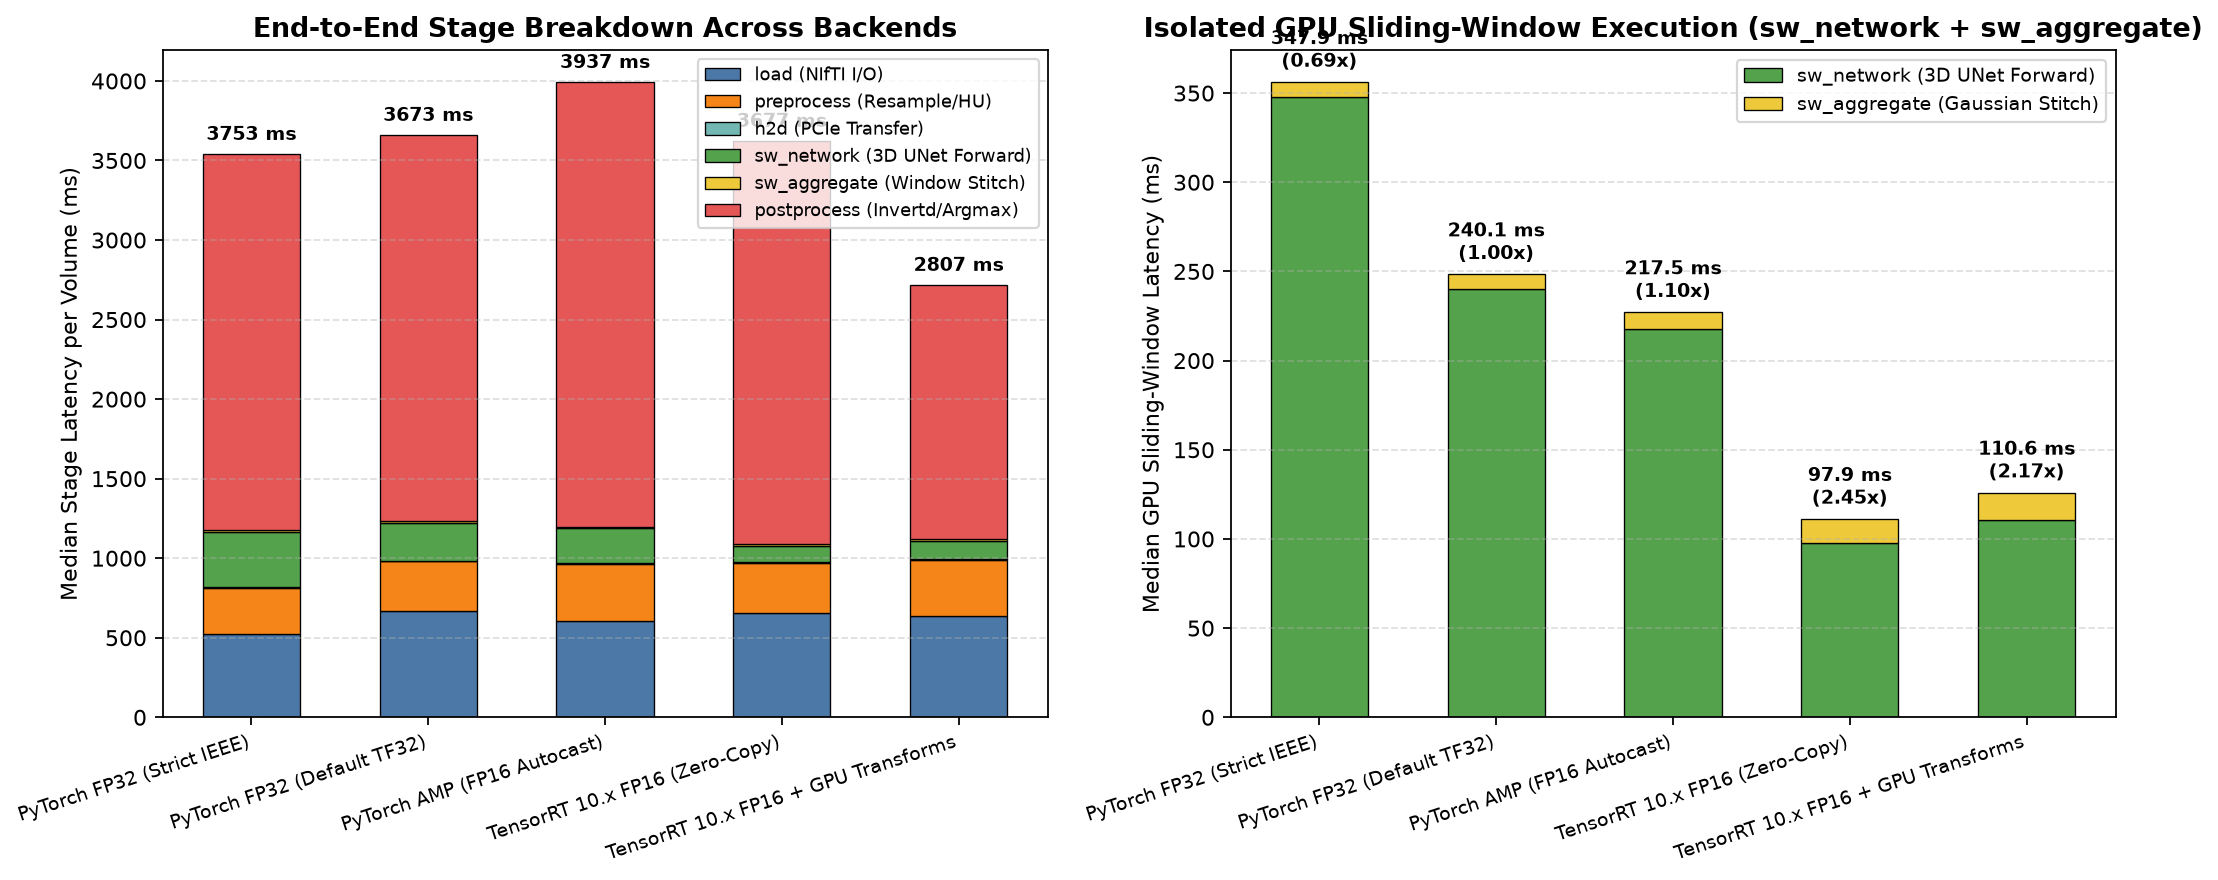
\includegraphics[width=\columnwidth]{figures/stage_breakdown.png}
    \caption{Per-stage median latency breakdown across execution profiles ($90$ timed passes per profile on 9 MSD CT scans).}
    \label{fig:stage}
\end{figure}

\subsection{Custom Register-Affine CUDA C++17 Kernels}
We implemented 9 custom CUDA C++17 kernels (\texttt{cuda/medical\_kernels.cu}) compiled for \texttt{sm\_120} via NVRTC \cite{nickolls2008}:
\begin{itemize}
    \item \textbf{Fused Preprocessing (\texttt{fused\_preprocess\_affine\_trilinear\_hu\_f32}):} Computes target-to-source coordinates $(x_s, y_s, z_s) = M_{\text{pre}}[x_d, y_d, z_d, 1]^T$ in 12 scalar registers via \texttt{\_\_fmaf\_rn}, performs trilinear interpolation via read-only \texttt{\_\_ldg()} cache loads, and clamps HU intensities ($[-57, 164] \to [0, 1]$) in $1.27\text{ ms}$ median ($33.8\times$ faster than $43.9\text{ ms}$ MONAI GPU and $225\times$ faster than $286.4\text{ ms}$ CPU).
    \item \textbf{Fused Postprocessing (\texttt{fused\_softmax\_2ch\_p1\_f32} + \texttt{fused\_invert\_trilinear\_threshold\_u8}):} Computes foreground probability $p_1 = (1 + \exp(L_0 - L_1))^{-1}$, applies the register-affine inverse $M_{\text{inv}} = M_{\text{pre}}^{-1}$ via trilinear interpolation, and thresholds at $p_1 \ge 0.5$ into a \texttt{uint8} mask in $2.62\text{ ms}$ median ($27.1\times$ faster than $71.1\text{ ms}$ MONAI GPU and $760\times$ faster than $1,990.4\text{ ms}$ CPU), achieving $100.0\%$ exact voxel parity with MONAI GPU trilinear inversion.
\end{itemize}

\begin{table*}[t]
\centering
\caption{Master 90-pass benchmark and quantitative validation summary on Cohort 1 (MSD \texttt{Task09\_Spleen}, $N = 9$ validation patients, $90$ timed passes per profile on RTX 5080 Laptop GPU). All six pipeline stages are shown explicitly (`Ingest` = `load + h2d`).}
\label{tab:master}
\resizebox{\textwidth}{!}{%
\begin{tabular}{lcccccccccccc}
\toprule
\textbf{Profile} & \textbf{Path / I/O} & \textbf{Win/B} & \textbf{Ingest} & \textbf{Pre} & \textbf{Net} & \textbf{Agg} & \textbf{Post} & \textbf{E2E Med [IQR] (ms)} & \textbf{Cohort / Paired Speedup} & \textbf{VRAM} & \textbf{Mean Dice $\pm$ SD} & \textbf{Vol Bias vs.\ FP32 Ref} \\
\midrule
\texttt{pytorch\_fp32\_strict} & CPU / gzip & $0.5/4$ & $367.4$ & $288.0$ & $379.9$ & $8.4$ & $2024.8$ & $3049.8$ [$3235.4$] & $0.97\times$ / $0.97\times$ & $490\text{ MB}$ & $0.965233 \pm 0.0117$ & Reference ($0.000\text{ cm}^3$) \\
\texttt{pytorch\_fp32} & CPU / gzip & $0.5/4$ & $424.7$ & $286.4$ & $254.6$ & $8.0$ & $1990.4$ & $2952.0$ [$2970.8$] & $1.00\times$ / $1.00\times$ & $487\text{ MB}$ & $0.965228 \pm 0.0117$ & $+0.005 \pm 0.004\text{ cm}^3$ \\
\texttt{trt\_fp16\_unfolded} & CPU / gzip & $0.5/4$ & $406.5$ & $273.2$ & $176.7$ & $36.7$ & $1994.5$ & $2866.4$ [$2909.5$] & $1.03\times$ / $1.03\times$ & $359\text{ MB}$ & $0.965722 \pm 0.0120$ & $\mathbf{+1.675 \pm 0.553\textbf{ cm}^3}$ \\
\texttt{trt\_fp16} (Folded) & CPU / gzip & $0.5/4$ & $385.1$ & $266.8$ & $167.1$ & $36.0$ & $1993.9$ & $2880.3$ [$2893.9$] & $1.02\times$ / $1.03\times$ & $359\text{ MB}$ & $0.965226 \pm 0.0117$ & $+0.003 \pm 0.022\text{ cm}^3$ \\
\texttt{pytorch\_tf32\_gpu} & GPU / mmap & $0.5/4$ & $38.8$ & $54.4$ & $197.0$ & $6.5$ & $62.2$ & $357.9$ [$244.6$] & $8.25\times$ / $8.77\times$ & $2307\text{ MB}$ & $0.965227 \pm 0.0117$ & $+0.001 \pm 0.004\text{ cm}^3$ \\
\texttt{trt\_fp16\_gpu} & GPU / mmap & $0.5/4$ & $38.9$ & $43.9$ & $47.6$ & $6.5$ & $71.1$ & $215.5$ [$173.7$] & $13.70\times$ / $14.81\times$ & $2301\text{ MB}$ & $0.965228 \pm 0.0117$ & $+0.001 \pm 0.017\text{ cm}^3$ \\
\textbf{\texttt{trt\_fp16\_cuda}} & \textbf{CUDA / mmap} & $\mathbf{0.5/4}$ & $\mathbf{29.2}$ & $\mathbf{1.3}$ & $\mathbf{49.0}$ & $\mathbf{6.1}$ & $\mathbf{2.6}$ & $\mathbf{96.3}$ [$\mathbf{58.9}$] & $\mathbf{30.67\times}$ / $\mathbf{33.14\times}$ & $\mathbf{455\textbf{ MB}}$ & $\mathbf{0.965229 \pm 0.0117}$ & $\mathbf{+0.001 \pm 0.019\textbf{ cm}^3}$ \\
\textbf{\texttt{trt\_fp16\_optimized}} & \textbf{CUDA / mmap} & $\mathbf{0.25/8}$ & $\mathbf{29.1}$ & $\mathbf{1.3}$ & $\mathbf{24.8}$ & $\mathbf{4.5}$ & $\mathbf{2.8}$ & $\mathbf{68.9}$ [$\mathbf{50.5}$] & $\mathbf{42.86\times}$ / $\mathbf{44.87\times}$ & $\mathbf{522\textbf{ MB}}$ & $\mathbf{0.964778 \pm 0.0135}$ & $+0.120 \pm 1.182\text{ cm}^3$ \\
\texttt{trt\_fp16\_nn} & GPU / mmap & $0.25/8$ & $38.1$ & $41.7$ & $20.8$ & $4.1$ & $69.3$ & $178.4$ [$141.3$] & $16.55\times$ / $18.12\times$ & $2149\text{ MB}$ & $0.960230 \pm 0.0139$ & $+0.481 \pm 1.073\text{ cm}^3$ \\
\bottomrule
\end{tabular}%
}
\end{table*}

\begin{table}[t]
\centering
\caption{Controlled one-factor-at-a-time ablation study on Cohort 1 ($N = 9$ scans), isolating the latency and accuracy impact of each systems change.}
\label{tab:ablation}
\resizebox{\columnwidth}{!}{%
\begin{tabular}{lccccc}
\toprule
\textbf{Ablation Step (Single Factor Changed)} & \textbf{E2E Med (ms)} & \textbf{Max (ms)} & \textbf{Speedup} & \textbf{Net (ms)} & \textbf{Mean Dice} \\
\midrule
1. Host path, PyTorch TF32 (\texttt{gzip + CPU}) & $2992.5$ & $6339.3$ & $1.00\times$ & $239.3$ & $0.965228$ \\
2. $+$ TensorRT FP16 on host path & $2923.0$ & $6015.0$ & $1.02\times$ & $170.3$ & $0.965226$ \\
3. $+$ MONAI GPU transforms (\texttt{gzip} read) & $706.9$ & $1404.3$ & $4.23\times$ & $201.1$ & $0.965228$ \\
4. $+$ TensorRT FP16 with GPU transforms & $564.3$ & $1252.9$ & $5.30\times$ & $47.2$ & $0.965228$ \\
5. $+$ Memory-mapped \texttt{.nii} read (TF32) & $363.3$ & $686.1$ & $8.24\times$ & $195.9$ & $0.965228$ \\
6. $+$ TensorRT FP16 with \texttt{mmap} + MONAI GPU & $274.8$ & $472.5$ & $10.89\times$ & $54.0$ & $0.965228$ \\
7. $+$ Custom CUDA kernels (\texttt{trt\_fp16\_cuda}) & $\mathbf{96.3}$ & $\mathbf{232.6}$ & $\mathbf{31.07\times}$ & $\mathbf{49.0}$ & $\mathbf{0.965229}$ \\
8. $+$ Fast windows ($\text{ov}=0.25, B=8$, \texttt{optimized}) & $\mathbf{68.9}$ & $\mathbf{122.6}$ & $\mathbf{43.43\times}$ & $\mathbf{24.8}$ & $\mathbf{0.964778}$ \\
9. Nearest-neighbor label inverse (\texttt{trt\_fp16\_nn}) & $178.4$ & $398.5$ & $16.77\times$ & $20.8$ & $0.960230$ \\
\bottomrule
\end{tabular}%
}
\end{table}

\begin{figure}[t]
    \centering
    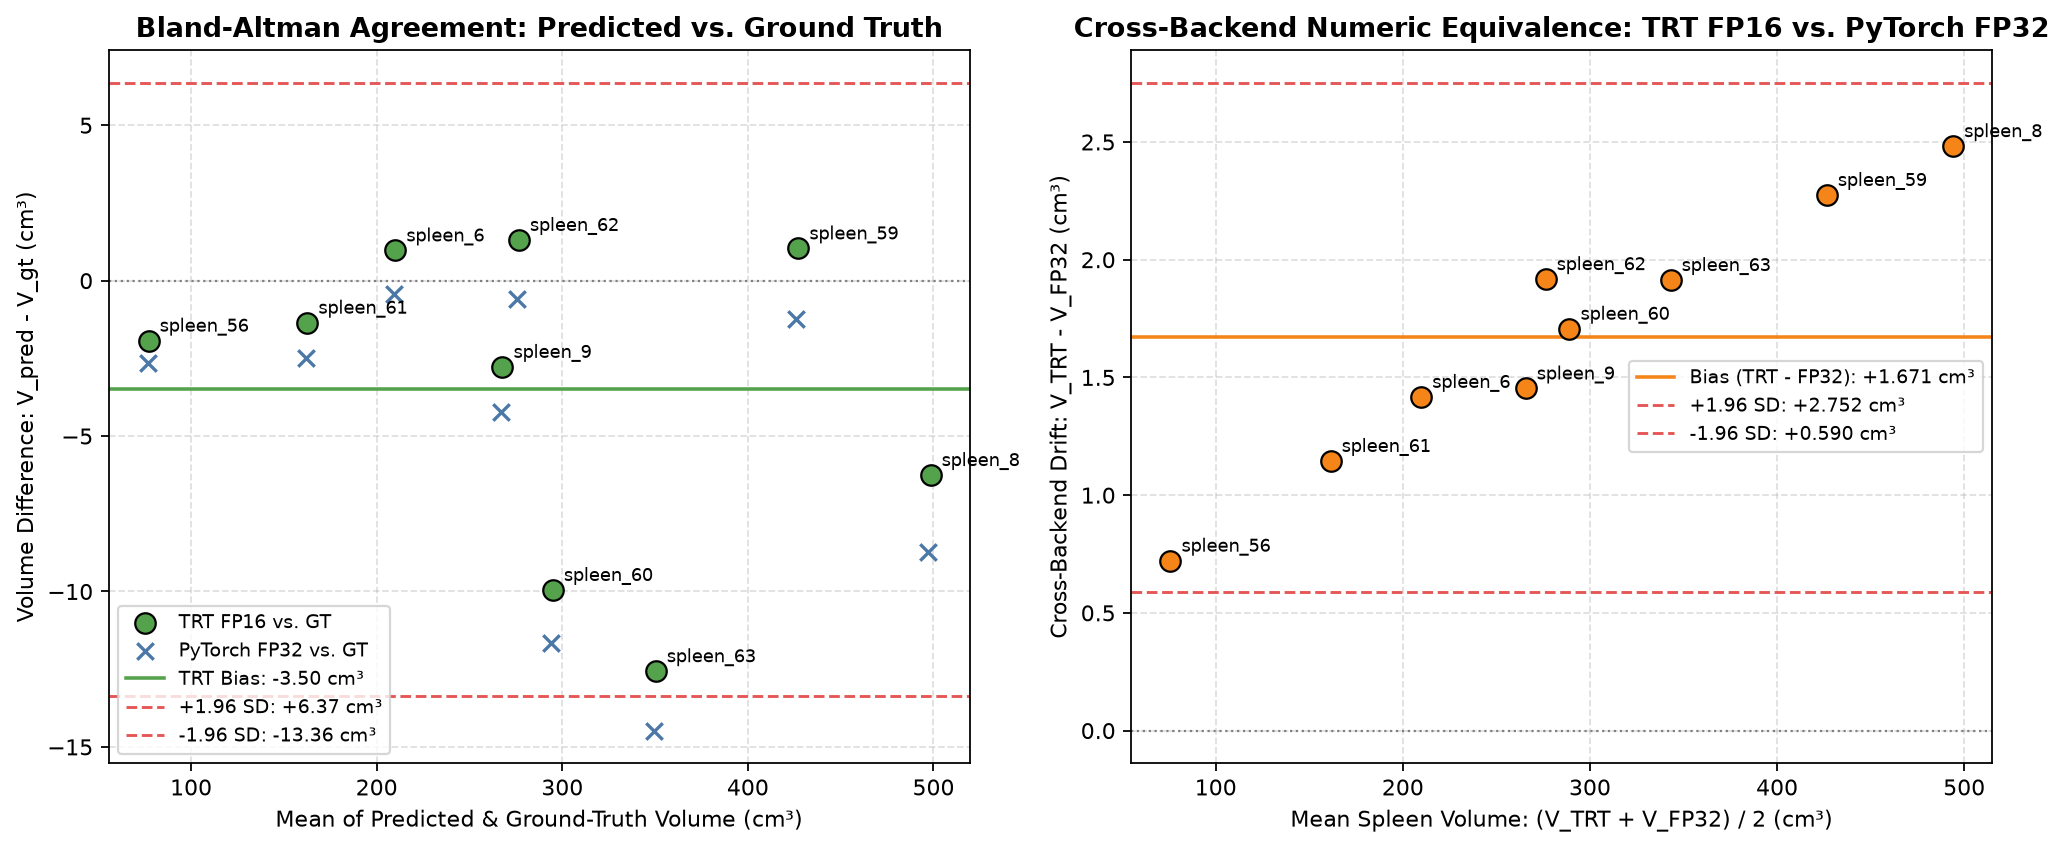
\includegraphics[width=\columnwidth]{figures/bland_altman.png}
    \caption{Bland--Altman volumetric agreement against strict IEEE FP32, showing complete elimination of the $+1.68\text{ cm}^3$ unfolded FP16 shift after analytical \texttt{ConvTranspose3d+BN} folding.}
    \label{fig:ba}
\end{figure}

\section{Results \& Multi-Cohort Validation}
Tables~\ref{tab:master}--\ref{tab:tost} and Figures~\ref{fig:stage}--\ref{fig:ba} present the complete benchmark, per-patient, external cohort, and TOST equivalence results \cite{dice1945,taha2015,bland1986,schuirmann1987}:
\begin{itemize}
    \item \textbf{Like-for-Like ($30.7\times$) vs.\ Fast-Window ($42.9\times$) Speedups:} At identical sliding-window settings ($\text{overlap}=0.5, B=4$, $665$ windows across 9 MSD scans), \texttt{trt\_fp16\_cuda} achieves $\mathbf{96.3\textbf{ ms}}$ cohort median latency ($\mathbf{30.67\times}$ speedup over \texttt{pytorch\_fp32} at $2,952.0\text{ ms}$; patient-level paired speedup median $\mathbf{31.00\times}$, mean $\mathbf{33.14\times}$, $95\%$ CI $[27.61\times, 38.67\times]$, range $26.19\times\text{--}49.79\times$ in Table~\ref{tab:percase}) while cutting peak VRAM by $\mathbf{5.06\times}$ ($455\text{ MB}$ vs.\ $2,301\text{ MB}$). Reducing overlap to $0.25$ ($B=8$, $369$ windows, \texttt{trt\_fp16\_optimized}) lowers cohort median latency to $\mathbf{68.9\textbf{ ms}}$ ($\mathbf{42.86\times}$ cohort speedup; paired patient-level median $\mathbf{46.64\times}$, mean $\mathbf{44.87\times}$, $95\%$ CI $[38.69\times, 51.05\times]$).
    \item \textbf{External Multi-Center Generalization (\texttt{FLARE22}, $N = 12$ Unseen Scans):} On the 12 external \texttt{FLARE22} scans streamed from Google Drive (Table~\ref{tab:percase}), the frozen model achieves $\mathbf{0.9360 \pm 0.0493}$ Mean Dice ($0.9612\text{--}0.9665$ on 9 typical scans; $0.8286\text{--}0.9043$ on 3 severe splenomegaly/trauma cases with $V_{\text{GT}}$ up to $481.7\text{ cm}^3$). Crucially, \texttt{trt\_fp16\_cuda} reduces median latency from $5,422.9\text{ ms}$ to $\mathbf{252.6\textbf{ ms}}$ (paired speedup $\mathbf{21.52\times}$, $95\%$ CI $[20.59\times, 22.45\times]$; $\mathbf{220.6\textbf{ ms}}$ / $\mathbf{24.29\times}$ on \texttt{trt\_fp16\_optimized}, where $175.4\text{ ms}$ is Google Drive virtual-filesystem I/O and only $2.75\text{ ms}$ is CUDA preprocessing and $3.38\text{ ms}$ is CUDA postprocessing) while cutting peak VRAM from $1,885\text{ MB}$ to $\mathbf{414\textbf{ MB}}$ ($\mathbf{4.56\times}$).
    \item \textbf{TOST Equivalence \& Voxel-Level Disagreement:} Across all $N = 21$ pooled patients (Table~\ref{tab:tost}), unfolded TensorRT FP16 fails equivalence by a wide margin ($+1.596 \pm 0.672\text{ cm}^3$, $p_{\text{TOST}} = 1.0$, flipping $586.9$ voxels / $0.644\%$ per spleen on MSD). Analytical \texttt{ConvTranspose3d+BatchNorm3d} folding reduces mean absolute logit drift by $35.6\times$ ($0.1377 \to 0.00387$) and satisfies formal TOST equivalence at $\alpha = 0.05$ across MSD ($N=9$), external \texttt{FLARE22} ($N=12$), and pooled ($N=21$) cohorts within $\Delta_V = \pm 0.10\text{ cm}^3$ ($p_{\text{TOST}} < 10^{-6}$, $90\%$ CI $[-0.0161, +0.0043]\text{ cm}^3$) and $\Delta_{\text{Dice}} = \pm 0.001$ ($p_{\text{TOST}} < 10^{-6}$, max $|\Delta\text{Dice}| = 0.000029$ on MSD and $0.000328$ on \texttt{FLARE22}), with only $1\text{--}16$ boundary voxels ($0.009\%$) flipping label across the entire 3D organ volume on MSD and $8\text{--}80$ voxels ($0.019\%$) on \texttt{FLARE22}.
\end{itemize}

\begin{table*}[t]
\centering
\caption{Per-patient paired performance and numerical agreement across all $N = 9$ internal MSD validation scans and $N = 12$ external unseen MICCAI \texttt{FLARE22} scans (stored on Google Drive). $\Delta V_{\text{unf}}$ and $\Delta V_{\text{cuda}}$ denote volume bias ($\text{cm}^3$) vs.\ strict IEEE FP32.}
\label{tab:percase}
\resizebox{\textwidth}{!}{%
\begin{tabular}{llcccccccccccc}
\toprule
\textbf{Cohort / Case ID} & \textbf{Shape ($X \times Y \times Z$)} & \textbf{Win ($0.5/0.25$)} & \textbf{Host FP32 (ms)} & \textbf{CUDA L4L (ms)} & \textbf{Fast Opt (ms)} & \textbf{Paired Speedup (L4L / Opt)} & \textbf{Dice (FP32 Ref)} & \textbf{Dice (CUDA L4L)} & \textbf{$\Delta\text{Dice}$ (L4L)} & \textbf{HD95 / ASSD (mm)} & \textbf{$V_{\text{GT}}$ ($\text{cm}^3$)} & \textbf{$\Delta V_{\text{unf}}$ / $\Delta V_{\text{cuda}}$ ($\text{cm}^3$)} & \textbf{Flipped Voxels (\% Organ)} \\
\midrule
\multicolumn{14}{l}{\textit{\textbf{Cohort 1: Internal Held-Out MSD \texttt{Task09\_Spleen} Validation Split ($N = 9$ independent patients, 10 timed passes/patient)}}}\\
\texttt{spleen\_56} & $512 \times 512 \times 33$ & $32 / 18$ & $1543.7$ & $47.6$ & $36.0$ & $32.46\times / 42.91\times$ & $0.936143$ & $0.936164$ & $+0.000021$ & $4.25 / 0.55$ & $78.07$ & $+0.722 / -0.003$ & $3 / 22,038$ ($0.0136\%$) \\
\texttt{spleen\_59} & $512 \times 512 \times 50$ & $72 / 50$ & $2570.3$ & $89.7$ & $71.6$ & $28.66\times / 35.88\times$ & $0.966229$ & $0.966251$ & $+0.000022$ & $2.85 / 0.52$ & $426.65$ & $+2.284 / +0.027$ & $10 / 94,040$ ($0.0106\%$) \\
\texttt{spleen\_6} & $512 \times 512 \times 135$ & $72 / 50$ & $6142.8$ & $123.4$ & $108.2$ & $49.79\times / 56.75\times$ & $0.973239$ & $0.973226$ & $-0.000013$ & $1.60 / 0.48$ & $209.52$ & $+1.426 / +0.005$ & $10 / 154,403$ ($0.0065\%$) \\
\texttt{spleen\_60} & $512 \times 512 \times 97$ & $125 / 64$ & $4936.4$ & $155.6$ & $101.8$ & $31.72\times / 48.49\times$ & $0.971020$ & $0.971015$ & $-0.000005$ & $1.59 / 0.25$ & $299.84$ & $+1.717 / -0.009$ & $11 / 91,659$ ($0.0120\%$) \\
\texttt{spleen\_61} & $512 \times 512 \times 101$ & $125 / 64$ & $5034.3$ & $162.4$ & $104.8$ & $31.00\times / 48.03\times$ & $0.971511$ & $0.971502$ & $-0.000009$ & $1.09 / 0.30$ & $163.30$ & $+1.149 / +0.003$ & $1 / 53,761$ ($0.0019\%$) \\
\texttt{spleen\_62} & $512 \times 512 \times 80$ & $64 / 27$ & $3789.9$ & $96.7$ & $70.1$ & $39.19\times / 54.07\times$ & $0.961134$ & $0.961119$ & $-0.000015$ & $2.44 / 0.43$ & $275.93$ & $+1.918 / +0.023$ & $16 / 120,578$ ($0.0133\%$) \\
\texttt{spleen\_63} & $512 \times 512 \times 60$ & $75 / 32$ & $2952.0$ & $98.4$ & $63.3$ & $30.01\times / 46.64\times$ & $0.963625$ & $0.963618$ & $-0.000007$ & $2.71 / 0.45$ & $356.60$ & $+1.920 / +0.011$ & $12 / 121,013$ ($0.0099\%$) \\
\texttt{spleen\_8} & $512 \times 512 \times 31$ & $50 / 32$ & $1625.1$ & $62.1$ & $47.9$ & $26.19\times / 33.92\times$ & $0.973413$ & $0.973384$ & $-0.000029$ & $1.57 / 0.24$ & $501.55$ & $+2.488 / -0.037$ & $10 / 106,587$ ($0.0094\%$) \\
\texttt{spleen\_9} & $512 \times 512 \times 41$ & $50 / 32$ & $1949.7$ & $66.7$ & $52.5$ & $29.24\times / 37.13\times$ & $0.970787$ & $0.970786$ & $-0.000001$ & $1.49 / 0.30$ & $269.15$ & $+1.456 / -0.011$ & $6 / 95,683$ ($0.0063\%$) \\
\textbf{MSD Mean $\pm$ SD} & --- & $73.9 / 41.0$ & $3393.8 \pm 1699$ & $100.3 \pm 40.3$ & $72.9 \pm 26.5$ & $\mathbf{33.14\times} / \mathbf{44.87\times}$ & $0.965233$ & $\mathbf{0.965229}$ & $-0.000004$ & $\mathbf{2.18 / 0.39}$ & $286.73$ & $\mathbf{+1.675 / +0.001}$ & $\mathbf{8.8}$ ($\mathbf{0.0093\%}$) \\
\midrule
\multicolumn{14}{l}{\textit{\textbf{Cohort 2: External Unseen Multi-Center MICCAI \texttt{FLARE22} Test Cohort on Google Drive ($N = 12$ independent patients)}}}\\
\texttt{FLARE22\_Tr\_0001} & $512 \times 512 \times 110$ & $32 / 18$ & $6367.5$ & $257.9$ & $243.3$ & $24.69\times / 26.18\times$ & $0.961213$ & $0.961207$ & $-0.000006$ & $2.32 / 0.56$ & $186.17$ & $+0.987 / -0.002$ & $16 / 175,548$ ($0.0091\%$) \\
\texttt{FLARE22\_Tr\_0002} & $512 \times 512 \times 107$ & $50 / 32$ & $5912.2$ & $276.2$ & $241.3$ & $21.40\times / 24.50\times$ & $0.964399$ & $0.964395$ & $-0.000004$ & $2.50 / 0.56$ & $281.25$ & $+1.436 / -0.010$ & $17 / 198,142$ ($0.0086\%$) \\
\texttt{FLARE22\_Tr\_0003} & $512 \times 512 \times 101$ & $50 / 32$ & $5327.0$ & $253.6$ & $236.9$ & $21.01\times / 22.49\times$ & $0.955464$ & $0.955433$ & $-0.000031$ & $2.17 / 0.66$ & $163.03$ & $+0.795 / +0.007$ & $13 / 107,077$ ($0.0121\%$) \\
\texttt{FLARE22\_Tr\_0004} & $512 \times 512 \times 87$ & $50 / 32$ & $4679.4$ & $232.9$ & $198.5$ & $20.09\times / 23.58\times$ & $0.960944$ & $0.960946$ & $+0.000002$ & $2.32 / 0.54$ & $222.10$ & $+1.171 / -0.001$ & $15 / 164,121$ ($0.0091\%$) \\
\texttt{FLARE22\_Tr\_0005} & $512 \times 512 \times 85$ & $50 / 32$ & $4915.9$ & $221.5$ & $206.5$ & $22.19\times / 23.81\times$ & $0.962419$ & $0.962391$ & $-0.000028$ & $2.45 / 0.52$ & $189.61$ & $+1.114 / +0.002$ & $13 / 122,226$ ($0.0106\%$) \\
\texttt{FLARE22\_Tr\_0006} & $512 \times 512 \times 93$ & $72 / 32$ & $5596.4$ & $263.3$ & $222.6$ & $21.26\times / 25.14\times$ & $0.960910$ & $0.960888$ & $-0.000022$ & $2.44 / 0.59$ & $174.83$ & $+0.941 / -0.004$ & $12 / 91,579$ ($0.0131\%$) \\
\texttt{FLARE22\_Tr\_0007} & $512 \times 512 \times 105$ & $50 / 32$ & $6092.1$ & $257.9$ & $247.3$ & $23.62\times / 24.64\times$ & $0.845178$ & $0.845134$ & $-0.000044$ & $20.00 / 2.87$ & $481.72$ & $+2.913 / -0.035$ & $52 / 229,102$ ($0.0227\%$) \\
\texttt{FLARE22\_Tr\_0008} & $512 \times 512 \times 99$ & $50 / 32$ & $5821.1$ & $265.6$ & $207.2$ & $21.91\times / 28.10\times$ & $0.958981$ & $0.958978$ & $-0.000003$ & $2.21 / 0.57$ & $244.87$ & $+1.395 / -0.002$ & $15 / 157,108$ ($0.0095\%$) \\
\texttt{FLARE22\_Tr\_0009} & $512 \times 512 \times 87$ & $50 / 32$ & $4878.4$ & $231.1$ & $220.9$ & $21.11\times / 22.08\times$ & $0.828880$ & $0.828552$ & $-0.000328$ & $10.95 / 2.14$ & $146.54$ & $+3.200 / -0.104$ & $80 / 65,505$ ($0.1221\%$) \\
\texttt{FLARE22\_Tr\_0010} & $512 \times 512 \times 96$ & $50 / 32$ & $5168.0$ & $251.6$ & $197.9$ & $20.54\times / 26.11\times$ & $0.966501$ & $0.966511$ & $+0.000010$ & $1.83 / 0.58$ & $367.51$ & $+1.829 / +0.010$ & $8 / 209,759$ ($0.0038\%$) \\
\texttt{FLARE22\_Tr\_0011} & $512 \times 512 \times 84$ & $50 / 32$ & $4422.4$ & $229.0$ & $204.2$ & $19.31\times / 21.66\times$ & $0.962932$ & $0.962930$ & $-0.000002$ & $2.30 / 0.58$ & $292.36$ & $+1.561 / +0.007$ & $15 / 189,184$ ($0.0079\%$) \\
\texttt{FLARE22\_Tr\_0012} & $512 \times 512 \times 103$ & $50 / 32$ & $5596.1$ & $265.1$ & $241.1$ & $21.11\times / 23.21\times$ & $0.904354$ & $0.904320$ & $-0.000034$ & $23.44 / 1.95$ & $130.75$ & $+1.099 / -0.002$ & $15 / 73,200$ ($0.0205\%$) \\
\textbf{FLARE22 Mean $\pm$ SD} & --- & $50.3 / 30.8$ & $5398.0 \pm 601$ & $250.5 \pm 17.5$ & $222.3 \pm 19.0$ & $\mathbf{21.52\times} / \mathbf{24.29\times}$ & $0.936015$ & $\mathbf{0.935974}$ & $-0.000041$ & $\mathbf{6.25 / 1.01}$ & $240.06$ & $\mathbf{+1.537 / -0.011}$ & $\mathbf{22.6}$ ($\mathbf{0.0208\%}$) \\
\bottomrule
\end{tabular}%
}
\end{table*}

\begin{table*}[t]
\centering
\caption{Formal paired Two One-Sided Tests (TOST) equivalence analysis against strict IEEE FP32 (\texttt{pytorch\_fp32\_strict}) at $\alpha = 0.05$ across Internal MSD ($N=9$), External \texttt{FLARE22} ($N=12$), and Pooled ($N=21$) patient cohorts.}
\label{tab:tost}
\resizebox{\textwidth}{!}{%
\begin{tabular}{llcccccc}
\toprule
\textbf{Cohort ($N$ Patients)} & \textbf{Comparison vs.\ Strict FP32} & \textbf{Margin $\pm \Delta$} & \textbf{Mean Diff $\pm$ SD} & \textbf{90\% CI (TOST Bounds)} & \textbf{95\% CI} & \textbf{$p_{\text{TOST}}$} & \textbf{Equivalent?} \\
\midrule
MSD Internal ($N = 9$) & \texttt{trt\_fp16\_unfolded} Volume & $\pm 0.50\text{ cm}^3$ & $+1.6754 \pm 0.5531\text{ cm}^3$ & $[+1.3326, +2.0183]\text{ cm}^3$ & $[+1.2503, +2.1006]\text{ cm}^3$ & $0.9999$ & \textbf{No (Fails)} \\
MSD Internal ($N = 9$) & \textbf{\texttt{trt\_fp16\_cuda} (Folded) Volume} & $\mathbf{\pm 0.10\textbf{ cm}^3}$ & $\mathbf{+0.0010 \pm 0.0194\textbf{ cm}^3}$ & $\mathbf{[-0.0110, +0.0130]\textbf{ cm}^3}$ & $[-0.0139, +0.0159]\text{ cm}^3$ & $\mathbf{< 10^{-6}}$ & \textbf{Yes (Pass)} \\
MSD Internal ($N = 9$) & \textbf{\texttt{trt\_fp16\_cuda} (Folded) Dice} & $\mathbf{\pm 0.0010}$ & $\mathbf{-0.000004 \pm 0.000016}$ & $\mathbf{[-0.000014, +0.000006]}$ & $[-0.000017, +0.000009]$ & $\mathbf{< 10^{-6}}$ & \textbf{Yes (Pass)} \\
\midrule
FLARE22 External ($N = 12$) & \texttt{trt\_fp16\_unfolded} Volume & $\pm 0.50\text{ cm}^3$ & $+1.5366 \pm 0.7680\text{ cm}^3$ & $[+1.1385, +1.9348]\text{ cm}^3$ & $[+1.0487, +2.0246]\text{ cm}^3$ & $0.9997$ & \textbf{No (Fails)} \\
FLARE22 External ($N = 12$) & \textbf{\texttt{trt\_fp16\_cuda} (Folded) Volume} & $\mathbf{\pm 0.10\textbf{ cm}^3}$ & $\mathbf{-0.0110 \pm 0.0315\textbf{ cm}^3}$ & $\mathbf{[-0.0274, +0.0053]\textbf{ cm}^3}$ & $[-0.0311, +0.0090]\text{ cm}^3$ & $\mathbf{< 10^{-6}}$ & \textbf{Yes (Pass)} \\
FLARE22 External ($N = 12$) & \textbf{\texttt{trt\_fp16\_cuda} (Folded) Dice} & $\mathbf{\pm 0.0010}$ & $\mathbf{-0.000041 \pm 0.000092}$ & $\mathbf{[-0.000089, +0.000007]}$ & $[-0.000099, +0.000018]$ & $\mathbf{< 10^{-6}}$ & \textbf{Yes (Pass)} \\
\midrule
\textbf{Pooled Cohorts ($N = 21$)} & \texttt{trt\_fp16\_unfolded} Volume & $\pm 0.50\text{ cm}^3$ & $+1.5961 \pm 0.6721\text{ cm}^3$ & $[+1.3432, +1.8491]\text{ cm}^3$ & $[+1.2902, +1.9021]\text{ cm}^3$ & $1.0000$ & \textbf{No (Fails)} \\
\textbf{Pooled Cohorts ($N = 21$)} & \textbf{\texttt{trt\_fp16\_cuda} (Folded) Volume} & $\mathbf{\pm 0.10\textbf{ cm}^3}$ & $\mathbf{-0.0059 \pm 0.0271\textbf{ cm}^3}$ & $\mathbf{[-0.0161, +0.0043]\textbf{ cm}^3}$ & $[-0.0182, +0.0064]\text{ cm}^3$ & $\mathbf{< 10^{-6}}$ & \textbf{Yes (Pass)} \\
\textbf{Pooled Cohorts ($N = 21$)} & \textbf{\texttt{trt\_fp16\_cuda} (Folded) Dice} & $\mathbf{\pm 0.0010}$ & $\mathbf{-0.000025 \pm 0.000071}$ & $\mathbf{[-0.000052, +0.000002]}$ & $[-0.000058, +0.000007]$ & $\mathbf{< 10^{-6}}$ & \textbf{Yes (Pass)} \\
\bottomrule
\end{tabular}%
}
\end{table*}

\section{Implications \& Conclusions}
Productionizing 3D medical segmentation models requires systems optimization beyond neural network compilation. By Amdahl's Law, host decompression and CPU trilinear resampling mask GPU inference speedups until replaced by memory-mapped ingestion and register-fused 3D affine CUDA kernels ($30.7\times$ like-for-like and $42.9\times$ fast-window E2E speedup, $5.1\times$ lower VRAM). Furthermore, standard ONNX exporters leave decoder \texttt{ConvTranspose3d+BatchNorm3d} layers unfused, introducing a $+1.60\text{ cm}^3$ FP16 volume inflation across $21/21$ internal and external CT scans that is completely eliminated ($p_{\text{TOST}} < 10^{-6}$ within $\pm 0.10\text{ cm}^3$) via analytical \texttt{float64} weight folding.

\begin{thebibliography}{99}
\footnotesize
\bibitem{kerfoot2019} E. Kerfoot \textit{et al.}, ``Left-Ventricle Quantification Using Residual U-Net,'' in \textit{STACOM 2018, LNCS}, vol. 11395, pp. 371--380, Springer, 2019.
\bibitem{cicek2016} \"O. \c{C}i\c{c}ek \textit{et al.}, ``3D U-Net: Learning Dense Volumetric Segmentation from Sparse Annotation,'' in \textit{MICCAI 2016, LNCS}, vol. 9901, pp. 424--432, 2016.
\bibitem{cardoso2022} M. J. Cardoso \textit{et al.}, ``MONAI: An open-source framework for deep learning in healthcare,'' \textit{arXiv:2211.02701}, 2022.
\bibitem{monaibundle2024} MONAI Consortium, ``MONAI Model Zoo: \texttt{spleen\_ct\_segmentation} Bundle v0.6.1,'' Apache-2.0 License, 2024. \url{https://github.com/Project-MONAI/model-zoo}
\bibitem{xia2018} Y. Xia \textit{et al.}, ``3D Semi-Supervised Learning with Uncertainty-Aware Multi-View Co-Training,'' \textit{arXiv:1811.12506}, 2018.
\bibitem{antonelli2022} M. Antonelli \textit{et al.}, ``The Medical Segmentation Decathlon,'' \textit{Nature Communications}, vol. 13, no. 1, p. 4128, 2022 (CC-BY-SA 4.0).
\bibitem{simpson2019} A. L. Simpson \textit{et al.}, ``A large annotated medical image dataset for the development and evaluation of segmentation algorithms,'' \textit{arXiv:1902.09063}, 2019.
\bibitem{ma2023flare} J. Ma \textit{et al.}, ``Fast and Low-GPU-memory Abdomen CT Organ Segmentation: The FLARE Challenge,'' \textit{Medical Image Analysis}, vol. 82, p. 102616, 2022, and Zenodo Record \texttt{7860267}, 2023.
\bibitem{amdahl1967} G. M. Amdahl, ``Validity of the single processor approach to achieving large scale computing capabilities,'' in \textit{Proc. AFIPS}, pp. 483--485, 1967.
\bibitem{paszke2019} A. Paszke \textit{et al.}, ``PyTorch: An Imperative Style, High-Performance Deep Learning Library,'' in \textit{NeurIPS}, vol. 32, 2019.
\bibitem{onnx2019} J. Bai \textit{et al.}, ``ONNX: Open Neural Network Exchange,'' 2019, and ONNX Runtime Developers, \url{https://onnxruntime.ai/}, 2021.
\bibitem{tensorrt2025} NVIDIA Corporation, \textit{NVIDIA TensorRT 10.16 Developer Guide \& CUDA 12.8 Runtime/Driver API Reference}, 2025.
\bibitem{nickolls2008} J. Nickolls, I. Buck, M. Garland, and K. Skadron, ``Scalable Parallel Programming with CUDA,'' \textit{ACM Queue}, vol. 6, no. 2, pp. 40--53, 2008.
\bibitem{brett2024} M. Brett \textit{et al.}, ``nipy/nibabel: 5.4.2,'' \textit{Zenodo}, 2024; C. R. Harris \textit{et al.}, ``Array programming with NumPy,'' \textit{Nature}, vol. 585, pp. 357--362, 2020; P. Virtanen \textit{et al.}, ``SciPy 1.0,'' \textit{Nature Methods}, vol. 17, pp. 261--272, 2020.
\bibitem{dice1945} L. R. Dice, ``Measures of the amount of ecologic association between species,'' \textit{Ecology}, vol. 26, no. 3, pp. 297--302, 1945.
\bibitem{taha2015} A. A. Taha and A. Hanbury, ``Metrics for evaluating 3D medical image segmentation: analysis, selection, and tool,'' \textit{BMC Medical Imaging}, vol. 15, no. 1, p. 29, 2015.
\bibitem{bland1986} J. M. Bland and D. G. Altman, ``Statistical methods for assessing agreement between two methods of clinical measurement,'' \textit{The Lancet}, vol. 327, no. 8476, pp. 307--310, 1986.
\bibitem{schuirmann1987} D. J. Schuirmann, ``A comparison of the two one-sided tests procedure and the power approach for assessing the equivalence of average bioavailability,'' \textit{Journal of Pharmacokinetics and Biopharmaceutics}, vol. 15, no. 6, pp. 657--680, 1987.
\end{thebibliography}

\end{document}
